\documentclass{beamer}

% Beamer style
\usetheme{CambridgeUS}
\usecolortheme[rgb={0.65,0.15,0.25}]{structure}
\beamertemplatenavigationsymbolsempty

% Packages
\usepackage[latin1]{inputenc}
\usepackage{color}
\usepackage{amsmath, amsfonts, amssymb}
\usepackage{marvosym}
\usepackage{graphicx}
\usepackage{/home/robin/LATEX/Biblio/astats}

% Commands
\definecolor{darkred}{rgb}{0.65,0.15,0.25}
\definecolor{darkgreen}{rgb}{0,0.4,0}
%\newcommand{\emphase}[1]{\textcolor{darkred}{#1}}
\newcommand{\Esp}{\mathbb{E}}
\newcommand{\dd}{\text{d}}
\newcommand{\emphase}[1]{{#1}}
\newcommand{\paragraph}[1]{\textcolor{darkred}{#1}}
\newcommand{\refer}[1]{\textcolor{gray}{\footnotesize{[\cite{#1}]}}}
\newcommand{\Refer}[1]{\textcolor{gray}{\footnotesize{[#1]}}}
\newcommand{\newblock}{}
\newcommand{\ra}{$\emphase{\rightarrow} \;$}

% Names
\newcommand{\chr}{}
\newcommand{\comment}{}

%====================================================================
\title[Genomic alterations]{Looking for recurrent genomic alterations: \\ A race against technologies}

\author[S. Robin]{S. Robin}

\institute[AgroParisTech / INRA]{
  \bigskip
 \begin{tabular}{ccccc}
    
\includegraphics[width=.2\textwidth]{../Figures/LogoINRA-Couleur} & 
    \hspace{.02\textwidth} &
    
\includegraphics[width=.3\textwidth]{../Figures/logagroptechsolo} & 
    \hspace{.02\textwidth} &
    
\includegraphics[width=.2\textwidth]{../Figures/logo-ssb} \\ 
  \end{tabular} \\
  \bigskip
  {\normalsize
    \begin{tabular}{rll}
    On-going work with & L. Decreusefond, & M.-P. Etienne, \\
    & G. Lang, & V. Stefanov \\
    \end{tabular}
    }
  }

  \date[MIA Jouy]{MIA Jouy, September 2014}

%====================================================================

%====================================================================
%====================================================================
\begin{document}
%====================================================================
%====================================================================

%====================================================================
\frame{\titlepage
  }
  
%====================================================================
\section*{Genomic alterations}
\frame{\frametitle{Genomic alterations}}
  
%====================================================================
\frame{\frametitle{Genomic alterations in cancer cells}

  $$
  \begin{tabular}{cc}
    \onslide+<1->{Normal cell} & \onslide+<2->{Tumor cell} \\
    \onslide+<1->{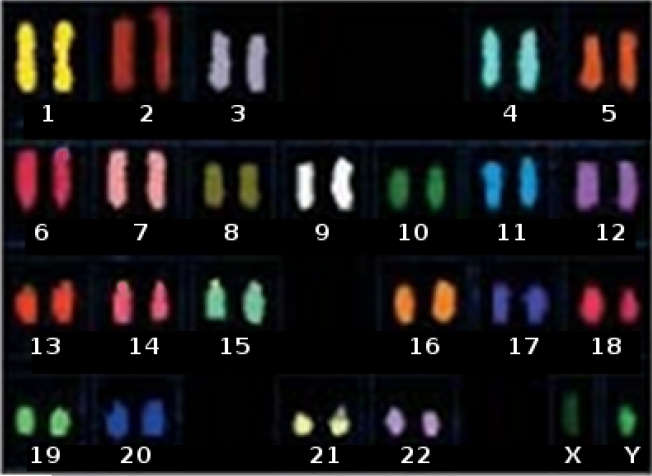
\includegraphics[height=.4\textheight]{../Figures/Hup08-Fig121b}}
    &
    \onslide+<2->{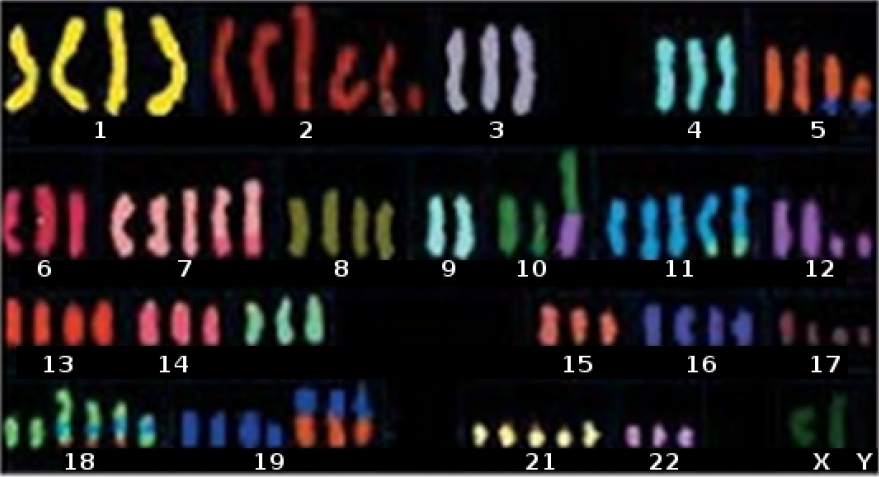
\includegraphics[height=.4\textheight]{../Figures/Hup08-Fig121a}}
  \end{tabular}
  $$
  \onslide+<2->{
  \refer{Hup08}
  }
}

%====================================================================
\frame{\frametitle{Detection of the alterations}

  $$
  \begin{tabular}{cc}
    Karyotype & {CGH profile}  \\
	 \\
    \begin{tabular}{l}
    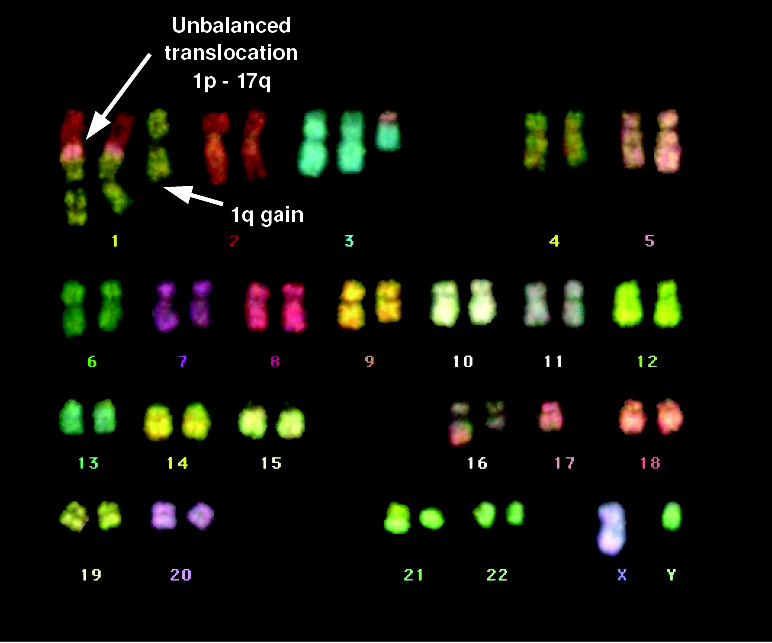
\includegraphics[height=.43\textheight]{../Figures/Hup08-Fig128b}
    \end{tabular}
    &
    \begin{tabular}{l}
    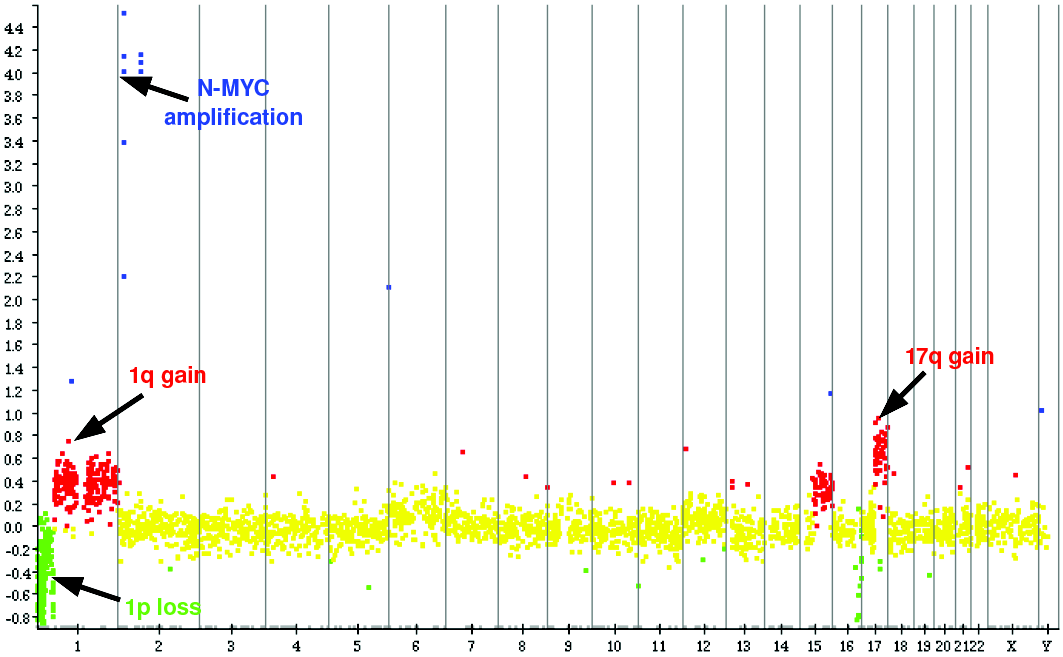
\includegraphics[height=.43\textheight]{../Figures/Hup08-Fig128a}
    \end{tabular}
  \end{tabular}
  $$
  \refer{Hup08}. 

}

%====================================================================
\frame{\frametitle{Recurrent alterations}

  \vspace{-.05\textheight}
  $$
  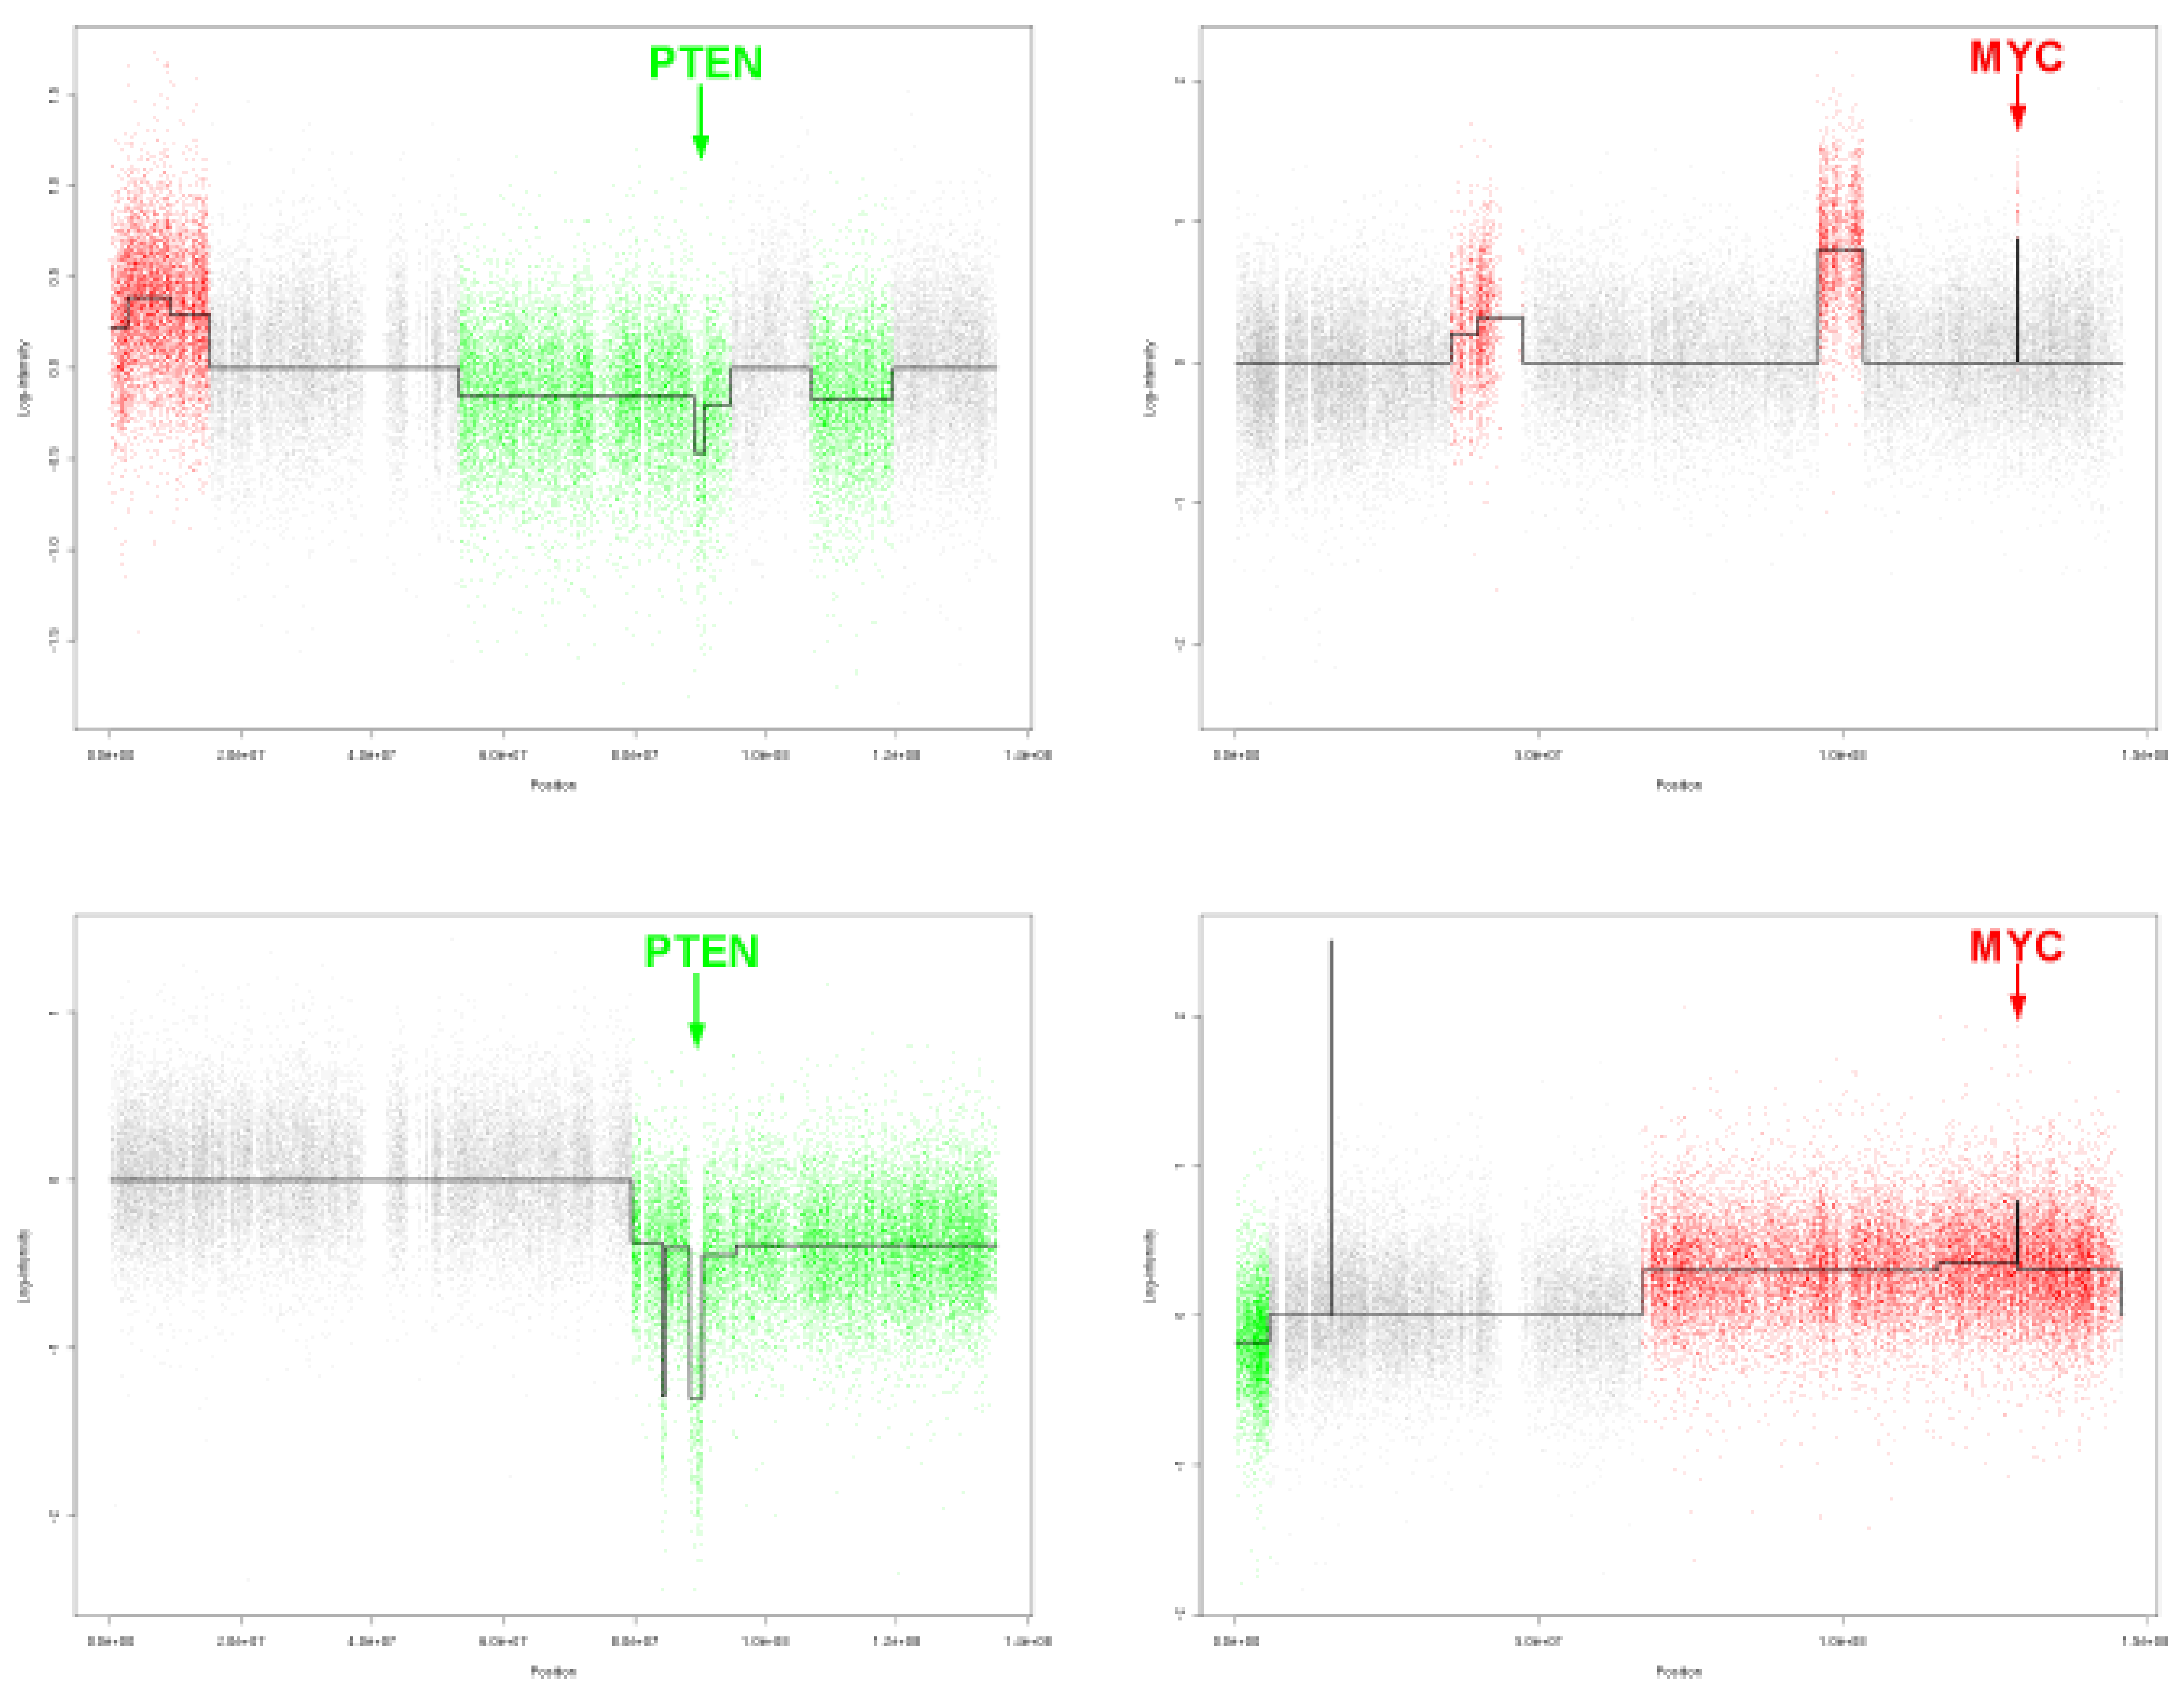
\includegraphics[height=.8\textheight]{../Figures/Rig10-Fig6-5}
  $$
  Chrom. 10 and 8 of two patients with breast carcinomas. \refer{Rig11} 
}

%====================================================================
\frame{\frametitle{Profiles}

  \begin{tabular}{cc}
    \begin{tabular}{p{0.5\textwidth}}
    \onslide+<1->{\paragraph{Individual profiles:} 
    patient $i$, locus $t$, 
    $$
    X_i(t) = \left\{
	 \begin{array}{ll}
	 0 & \text{if normal} \\
	 1 & \text{if \textcolor{red}{altered}}
	 \end{array}
    \right.
    $$
   }
    \onslide+<2->{\paragraph{Cumulated profile:}
    $$
    S(t) = \sum_{i=1}^p X_i(t)
    $$
    $= $ nb of altered patients at locus $t$ \\
   }
    \onslide+<3->{\bigskip
    \paragraph{Significance:}}
    \end{tabular}
    &
    \hspace{-0.1\textwidth}
    \begin{tabular}{c}
	 \begin{overprint}   
%	 \onslide<1>    
%	 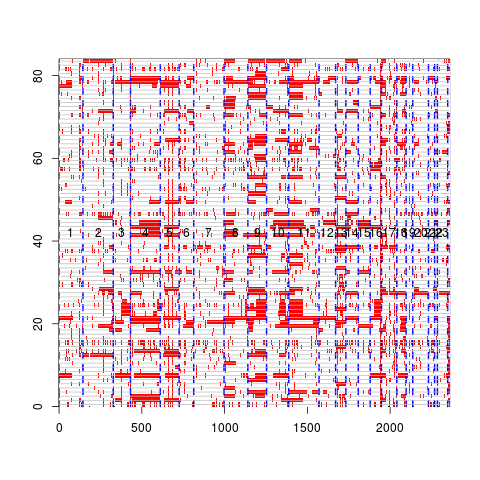
\includegraphics[height=.7\textheight, width=.5\textwidth]{../Figures/Fig-MinReg-Data-Prof} 
% 	 \onslide<2>    
% 	 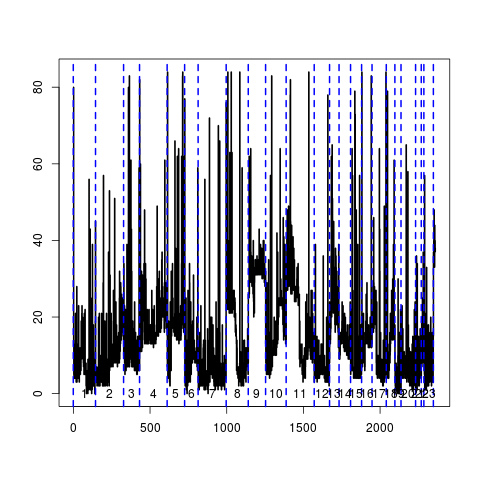
\includegraphics[height=.7\textheight, width=.5\textwidth]{../Figures/Fig-MinReg-Data-Cumul} 
	 \onslide<1>    
	 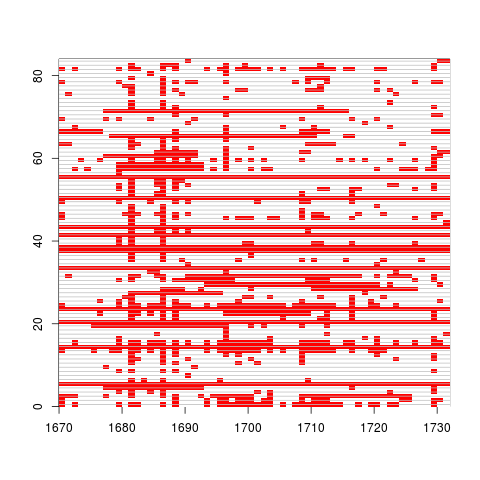
\includegraphics[height=.7\textheight, width=.5\textwidth]{../Figures/Fig-MinReg-Data-Prof13} 
	 \onslide<2>    
	 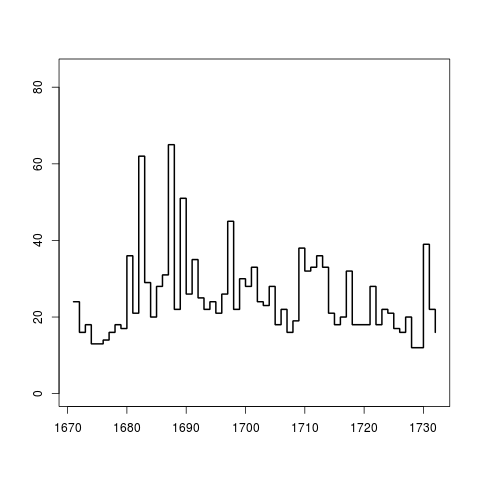
\includegraphics[height=.7\textheight, width=.5\textwidth]{../Figures/Fig-MinReg-Data-Cumul13} 
	 \onslide<3>    
	 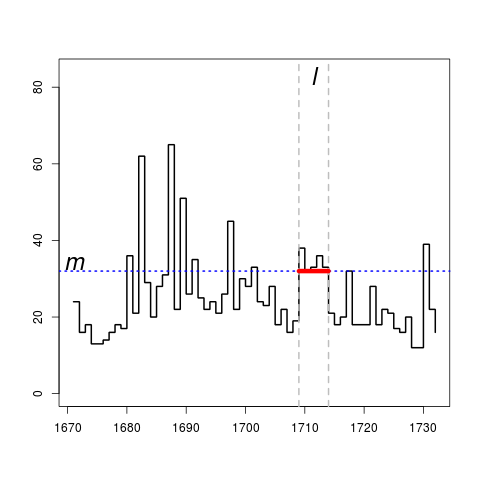
\includegraphics[height=.7\textheight, width=.5\textwidth]{../Figures/Fig-MinReg-Data-Reg1-13} 
	 \onslide<4>    
	 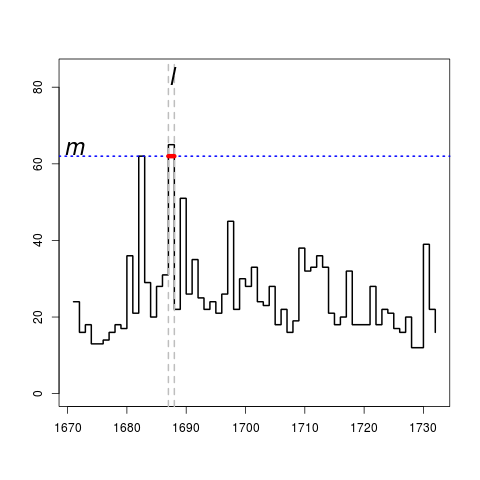
\includegraphics[height=.7\textheight, width=.5\textwidth]{../Figures/Fig-MinReg-Data-Reg2-13} 
	 \end{overprint}   
    \end{tabular}
  \end{tabular}
  \onslide+<3->{
  $$
  \pi(m, \ell) = \Pr\left\{\text{
  an excursion with length $\ell$ above level $m$ occurs
  }\right\}
  $$}

  }

%====================================================================
\frame{\frametitle{Generic model}

  \paragraph{Individual profiles.} Define a (Markov) model for each profile $X_i(t)$:
  $$
  X_i(t) \text{ iid } \sim F(\theta) 
  $$
  $\theta = $ e.g. alteration typical length and frequency.
  
  \bigskip \bigskip \pause
  \paragraph{Cumulated profiles.} Deduce the distribution of $S(t)$
  $$
  S(t) \sim G(\theta)
  $$
  
  \bigskip \pause
  \paragraph{Significance.} Compute the probability for $S(t)$ to stay above the threshold $m$ for longer than $\ell$:
  $$
  \pi(m, \ell) =
  \Pr\{\exists t \in ]\ell, n], \forall u \in ]t-\ell, t], S(u) \geq m\}
  $$
}

%====================================================================
\frame{\frametitle{Abacus}

  \paragraph{Significance isolines:} for given sample size $p$, number of loci $n$ and parameter $\theta \approx $ (mean nb. alterations, mean alteration length)
  $$
  \mathcal{C}_\alpha(\theta) = \{(m, \ell): \pi(m, \ell) = \alpha\}
  $$
  (e.g. $\alpha = 1\%$) \vspace{-.1\textheight}
  $$
  \begin{array}{rc}
    \begin{array}{c} \rotatebox{90}{threshold $m$} \end{array} & 
    \begin{array}{c} 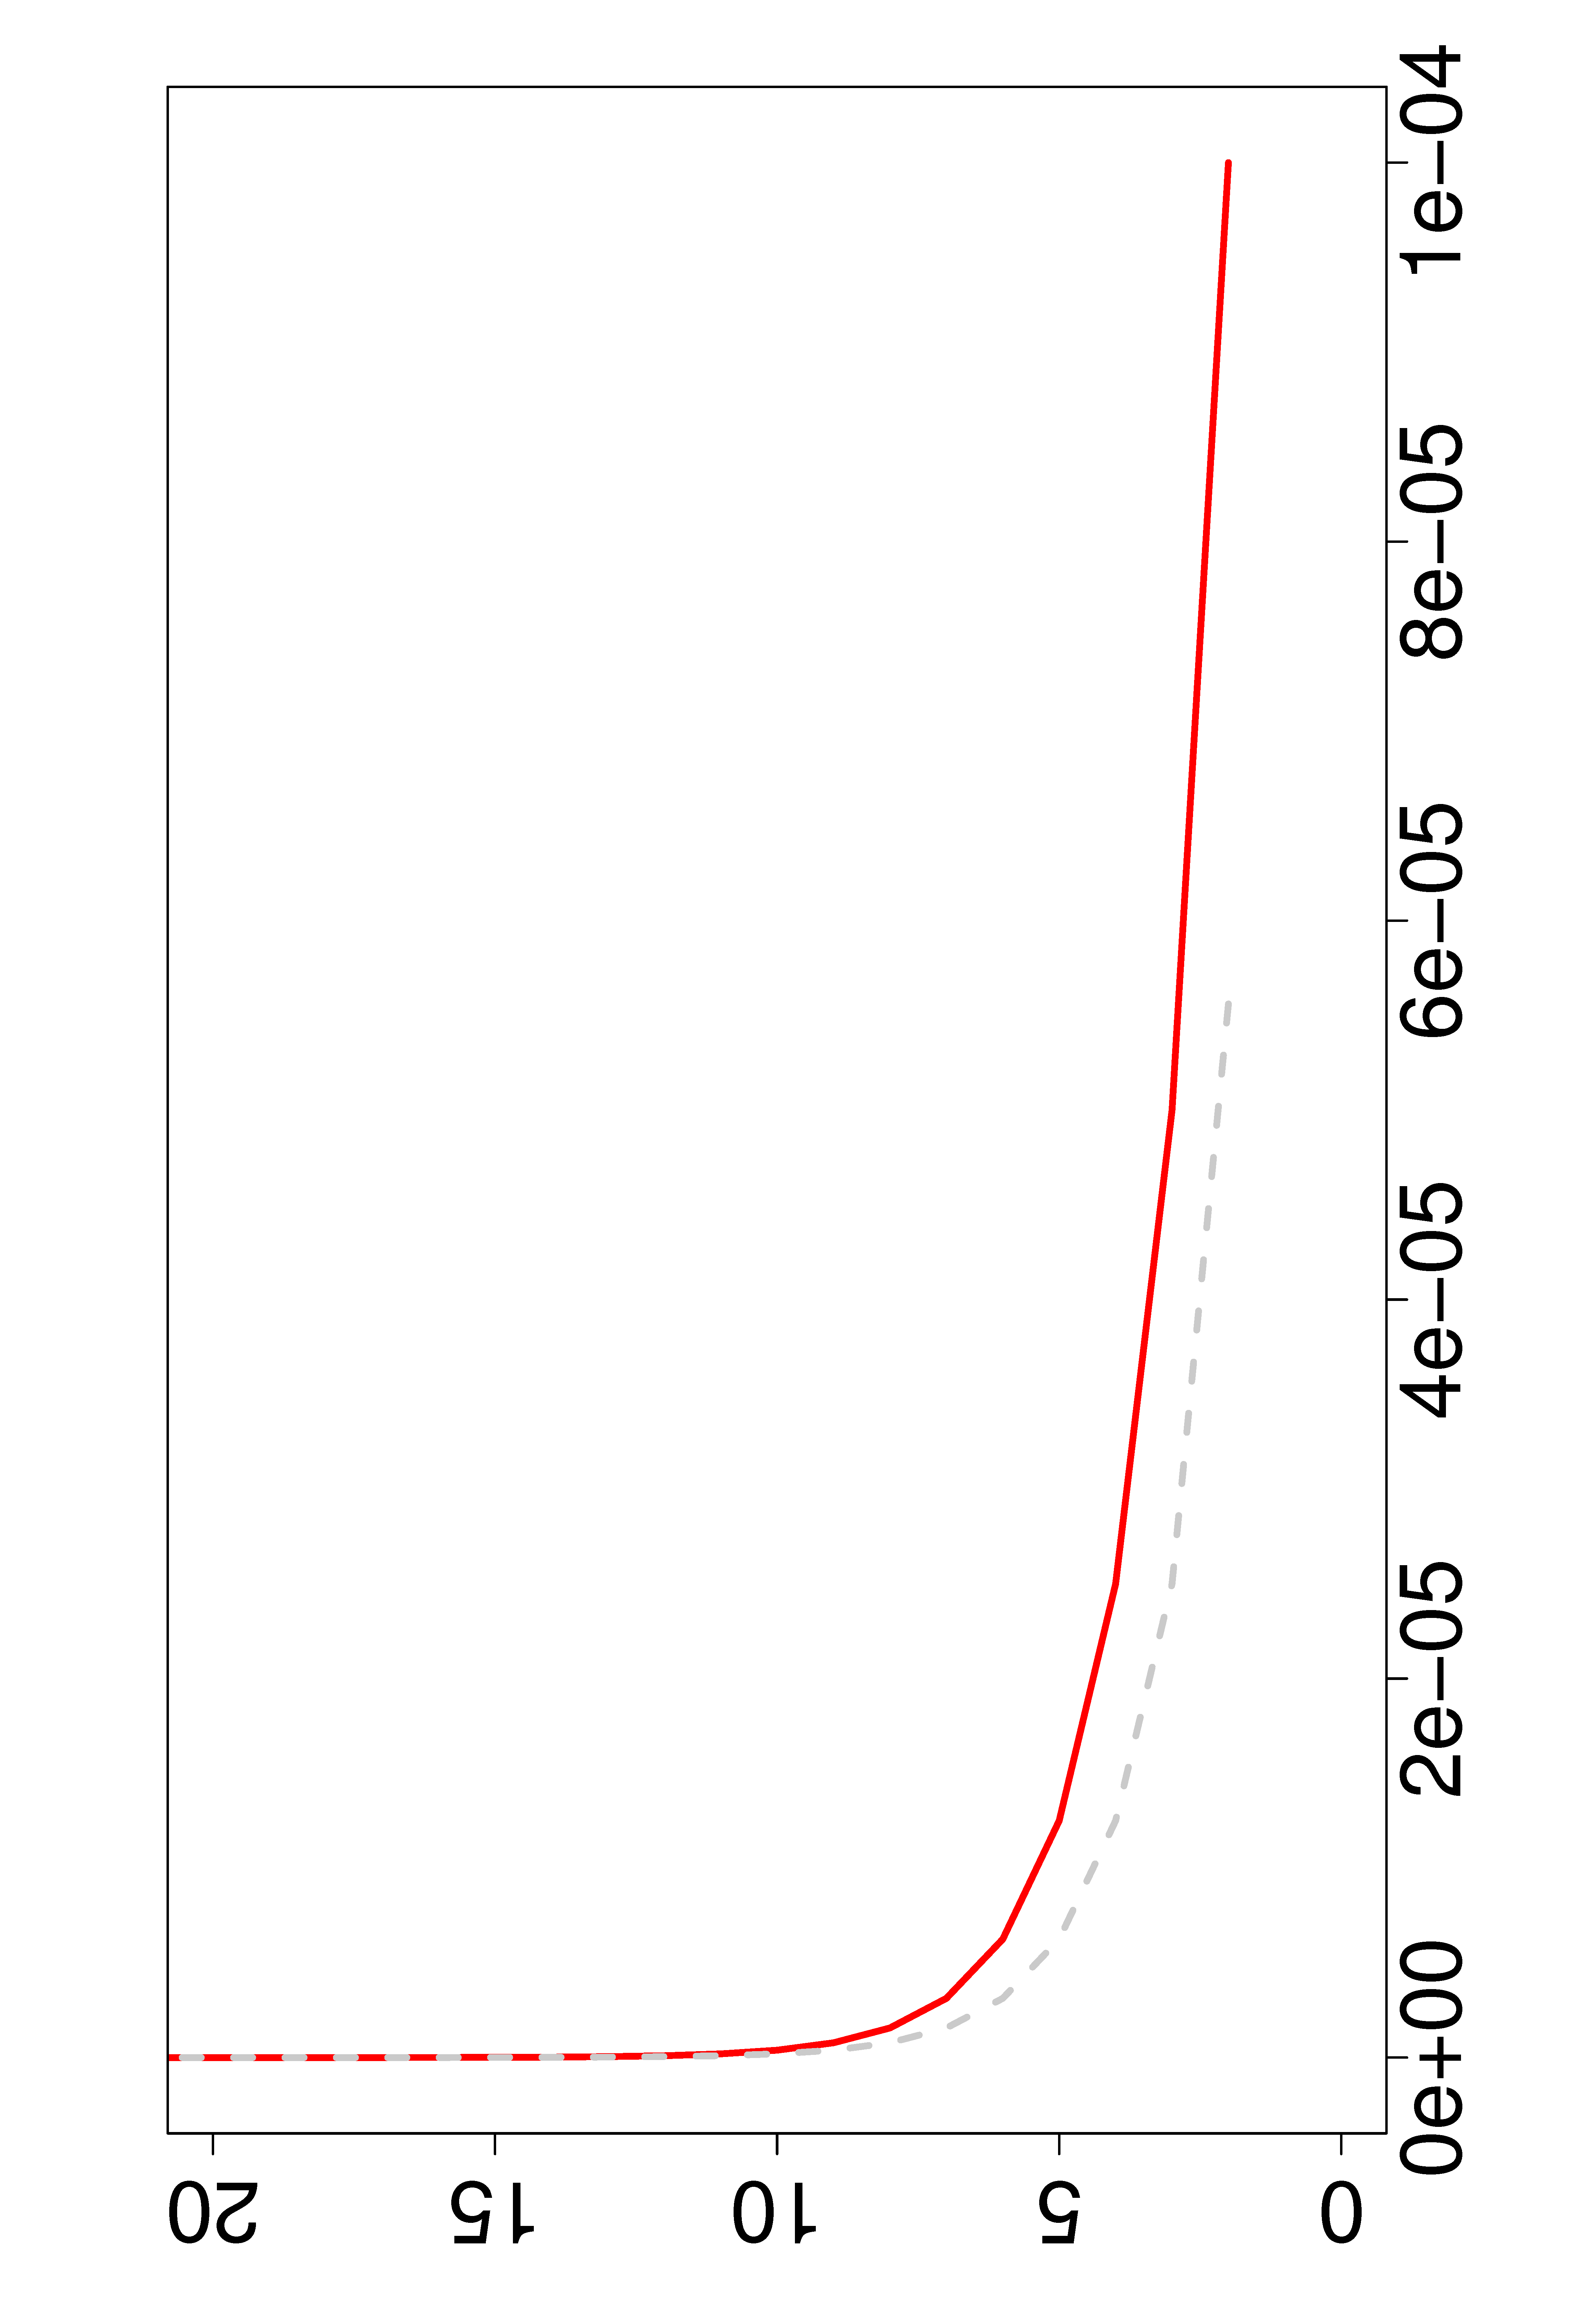
\includegraphics[height=.7\textheight, width=.45\textwidth, angle=270]{../Figures/Abaque-Example} \end{array} \\
    & \text{relative alteration length } \ell / n
  \end{array}
  $$
}

%====================================================================
\frame{\frametitle{Outline: A race vs technologies}

  \tableofcontents
  
}

  
%====================================================================
\section{Few loci, few patients}
\frame{\frametitle{Few loci, few patients}}
  
%====================================================================
\frame{\frametitle{Few loci, few patients}

  \paragraph{Mid 90' - early 00':} BAC arrays
  \begin{itemize}
   \item $10^3$ loci per array, $10^2$ loci per chromosome.
   \item Several k\EUR~per patient
  \end{itemize}
  
  \bigskip
  \paragraph{Data size:} 
  \begin{itemize}
   \item $n \approx 10^2$ loci
   \item $p \approx 10 - 10^2$ patients
  \end{itemize}
  
  \bigskip
  Joint work with V. Stefanov \Refer{R. and Stefanov (2009)}\nocite{RoS09}
}
  
%====================================================================
\frame{\frametitle{Discrete time Markov chain model}

  \paragraph{Individual profile.} $\{X_i(t)\}_i$ iid Markov chains over $\{0, 1\}$:
  $$
  X_i(t) \sim MC(P_X), 
  \qquad
  P_X = \left( 
    \begin{array}{cc} 1 - \lambda & \lambda \\ \mu & 1-\mu \end{array}
  \right).
  $$
  \ra Mean alteration length $= 1/ \mu$, one alteration every $\lambda\mu/(\lambda+\mu)$ locus.
  
  \bigskip \bigskip \pause
  \paragraph{Cumulated profile.} $S(t)$ is a Markov chain over $\{0, \dots, p\}$ with transition
  $$
  S(t+1) | S(t) \quad \overset{\Delta}{=} \quad \underset{\text{stay altered}}{\mathcal{B}\left(S(t), 1-\mu \right)} \; + \; \underset{\text{become altered}}{\mathcal{B}\left(p-S(t), \lambda \right)}
  $$
  \ra Transition matrix $P_S: (p+1) \times (p+1)$
}

%====================================================================
\frame{\frametitle{Embedded Markov chain}

  \paragraph{Aim = compute $\pi(m, \ell)$.}
  Define the stopping time 
  $$
  T(m, \ell) = \inf\{t: \forall u \in ]t-\ell, t], S(u) \geq m\},
  $$
  we have
  $$
  \pi(m, \ell) = \Pr\{T(m, \ell) \leq n\}.
  $$
  
  \bigskip \pause
  \paragraph{Embedded MC principle.} 
  \begin{itemize}
  \item Related to finite automata.
  \item Construct another Markov chain (with larger transition matrix $\widetilde{P}_S$) with absorbing state that is reached at the stopping time \refer{FuL03}. 
  \item In this case: relabel the states above $m$ to keep track of how long $S(t)$ has sojourned above $m$.
  \end{itemize}
}

%====================================================================
\frame{\frametitle{Constructing the waiting time}
  
  \paragraph{Automaton view-point.} $\ell = 4$:
  $$
  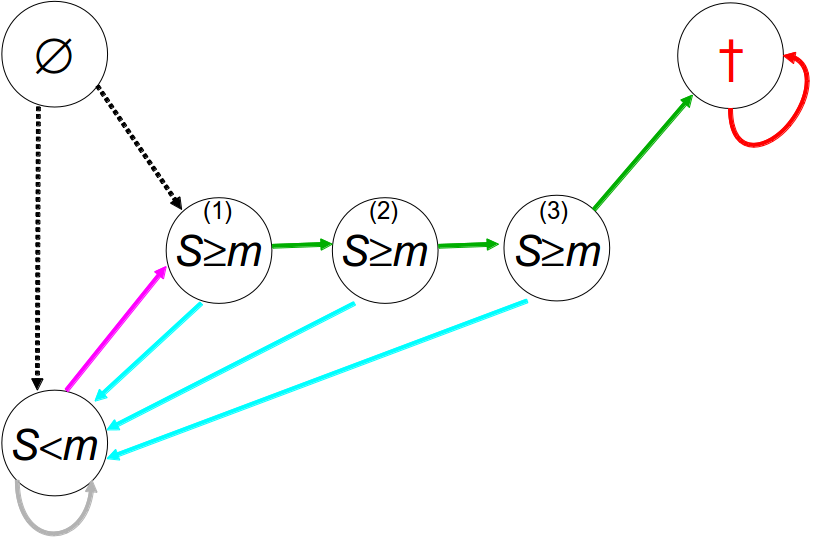
\includegraphics[height=.5\textheight, clip=]{../Figures/Fig-MinReg-Automaton}
  $$
  \ra We are left with the construction of the transition matrix $\widetilde{P}_S$ of this automaton.
}
%====================================================================
\frame{\frametitle{Constructing $\widetilde{P}_S$}

%   \vspace{-.08\textheight}
  \begin{tabular}{cc}
    \begin{tabular}{p{0.3\textwidth}}
	 \paragraph{Example.}
	 $$
	 p = 20, m = 15, \ell = 4
	 $$

	 \onslide+<6->{
	 \bigskip
	 \paragraph{Result.}
	 $$
	 \pi(m, \ell) = \left[\widetilde{P}_S^{n-1}\right]_{S(1), \textcolor{red}{\mathbf{\dagger}}}
	 $$
	 ($\textcolor{red}{\mathbf{\dagger}} = $ 'coffin state') \\ ~
	 \\ ~\\
	 or, if $S(1) \sim \nu$, \\
	 $\pi(m, \ell) = \left[\nu^\top \widetilde{P}_S^{n-1}\right]_{\textcolor{red}{\mathbf{\dagger}}}$ 
	 }
    \end{tabular}
    &
%    \hspace{-0.05\textwidth}
    \begin{tabular}{c}
	 \begin{overprint}   
	 \onslide<1>  
	 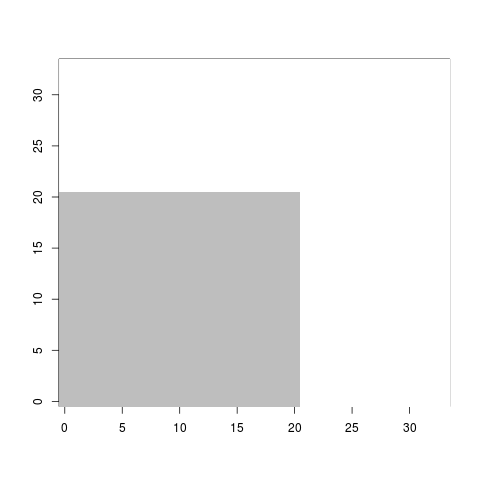
\includegraphics[height=.7\textheight]{../Figures/Fig-MinReg-EmbMC-Porg} \\
	 {\footnotesize $\{0, \dots, p\}$}
	 \onslide<2>    
	 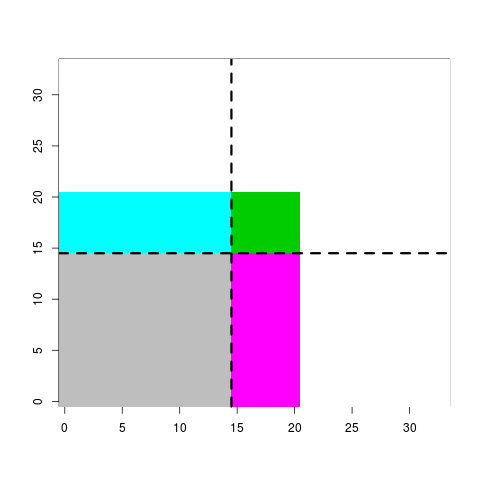
\includegraphics[height=.7\textheight]{../Figures/Fig-MinReg-EmbMC-Thres} \\
	 {\footnotesize $\{0, \dots, m-1, \underbrace{m, \dots, p}\}$}
	 \onslide<3>    
	 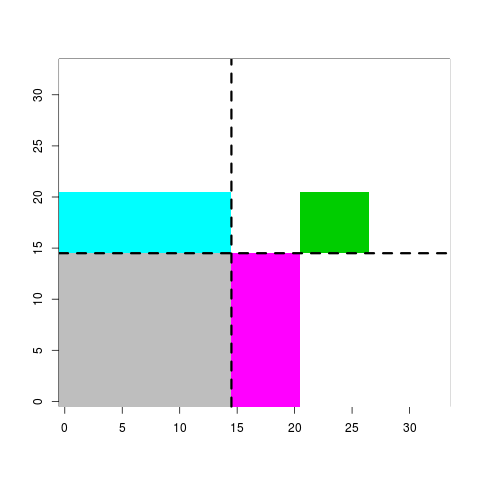
\includegraphics[height=.7\textheight]{../Figures/Fig-MinReg-EmbMC-1st} \\
	 {\footnotesize $\{0, \dots, m-1, \underbrace{m, \dots, p}, \underbrace{m', \dots, p'}\}$}
	 \onslide<4>    
	 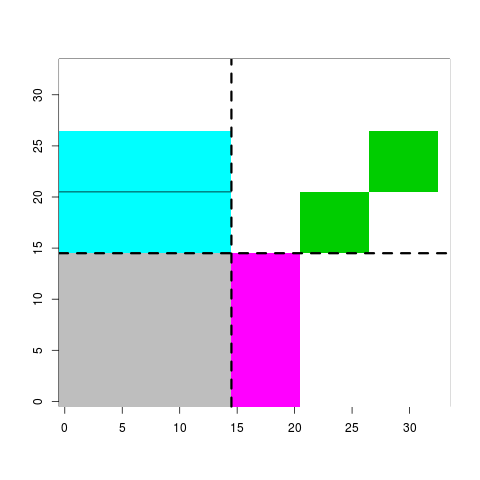
\includegraphics[height=.7\textheight]{../Figures/Fig-MinReg-EmbMC-2nd} \\
	 {\footnotesize $\{0, \dots, m-1, \underbrace{m, \dots, p}, \underbrace{m', \dots, p'}, \underbrace{m'', \dots, p''}\}$}
	 \onslide<5>    
	 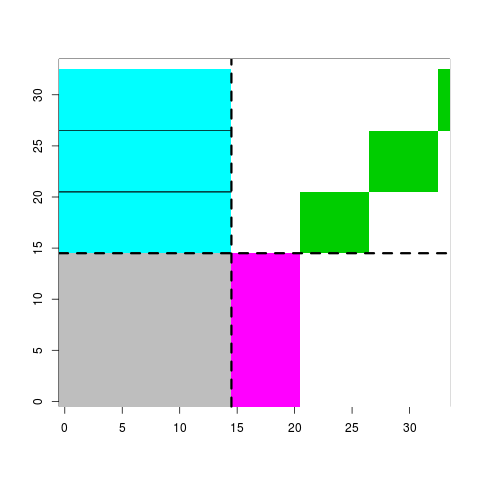
\includegraphics[height=.7\textheight]{../Figures/Fig-MinReg-EmbMC-3rd} \\
	 {\footnotesize $\{0, \dots, m-1, \underbrace{m, \dots, p}, \underbrace{m', \dots, p'}, \underbrace{m'', \dots, p''}, \textcolor{red}{\mathbf{\dagger}}\}$}
	 \onslide<6->   
	 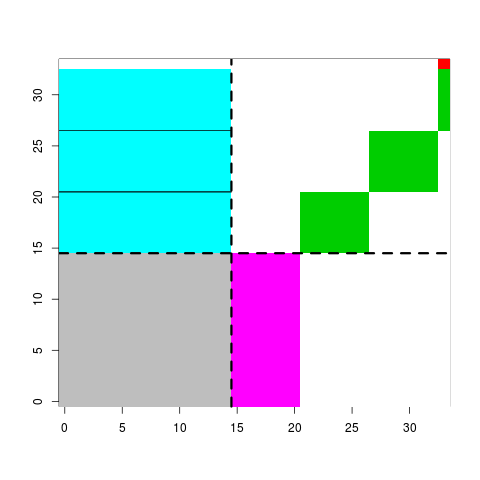
\includegraphics[height=.7\textheight]{../Figures/Fig-MinReg-EmbMC-Abs} \\
	 {\footnotesize $\{0, \dots, m-1, \underbrace{m, \dots, p}, \underbrace{m', \dots, p'}, \underbrace{m'', \dots, p''}, \textcolor{red}{\mathbf{\dagger}} \}$}
	 \end{overprint}   \\~
    \end{tabular}
  \end{tabular}
  
%   \onslide+<6>{
% %   \vspace{-0.1\textheight}
%   \ra Just need to compute $\widetilde{P}_S^{n-1}$.
%   }

  
%  \onslide+<7>{
%  \bigskip 
%  or, if $S(i) \sim \nu$,
%  $$
%  \pi(m, \ell) = \sum_s \nu(s) \pi_s(m, \ell) = \left[\nu^\top \widetilde{P}_S^{n-1}\right]_{\textcolor{red}{\mathbf{\dagger}}}
%  $$
%  }

  }

%====================================================================
\frame{\frametitle{(Provisional) conclusion}

  \paragraph{Ok:}
  \begin{itemize}
  \item Simple \& intuitive model,
  \item Exact result,
  \item Calculation easy to implement.
  \end{itemize}

  \pause \bigskip \bigskip
  \paragraph{But:}
  \begin{itemize}
  \item The embedded transition matrix $\widetilde{P}_S$ has dimension $\approx \ell \times p$ \\
  \ra not tractable for large population size $p$ and/or large alteration length $\ell$
  \item Computing its $(n-1)$-th power leads to numerical troubles for large number of loci $n$. 
  \end{itemize}

  }

%====================================================================
\section{Many loci, few patients}
\frame{\frametitle{Many loci, few patients}}
  
%====================================================================
\frame{\frametitle{Many loci, few patients}

  \paragraph{Mid 00':} %CGH arrays, 
  SNP arrays
  \begin{itemize}
   \item $10^5-10^6$ loci per array, $10^4-10^5$ loci per chromosome.
   \item Less than 1 k\EUR~per patient
  \end{itemize}
  
  \bigskip
  \paragraph{Data size:} 
  \begin{itemize}
   \item $n \approx 10^4-10^5 \rightarrow \infty$ loci
   \item $p \approx 10^2$ patients
  \end{itemize}
  
  \bigskip
  Joint work with V. Stefanov \Refer{R. and Stefanov (2013)}\nocite{RoS13}
}
  
%====================================================================
\frame{\frametitle{Continuous time Markov process}

  \paragraph{Individual profile.} $\{X_i(t)\}_i$ iid Markov processes over $\{0, 1\}$ with rates
  $$
  \begin{array}{lll}
   \text{alteration start} & 0 \rightarrow 1: & \lambda \\
   \text{alteration end} & 1 \rightarrow 0: & \mu
  \end{array}
  $$
  \ra Mean alteration length $= 1/ \mu$, alteration frequency $=\lambda\mu/(\lambda+\mu)$.
  
  \bigskip \bigskip \pause
  \paragraph{Cumulated profile.} $S(t)$ is a birth and death process over $\{0, \dots, p\}$ with rates
  $$
  \begin{array}{llrcl}
    \text{alteration 'birth'} & s \rightarrow s+1: & \lambda_s & = & \lambda \times (p-s)\\
    \text{alteration 'death'} & s \rightarrow s-1: & \mu_s & = & \mu \times s
  \end{array}
  $$
  \ra infinitesimal generator (transition rates) $Q: (p+1) \times (p+1)$. \\
  \bigskip \pause
  But we cannot 'count' the steps above the threshold anymore.
}

%====================================================================
\frame{\frametitle{Construction of the stopping time}

  \begin{tabular}{cc}
    \begin{tabular}{p{0.3\textwidth}}
 	 \onslide+<1->{$\ell = .05$} \\
 	 \onslide+<2->{$A = T_{S(0) \rightarrow m}$} \\
	 \onslide+<3->{$B = (T_{m \rightarrow m-1} | < \ell)$} \\
	 \onslide+<4->{$C = T_{m-1 \rightarrow m}$} \\
    \end{tabular}
    &
    \hspace{-0.1\textwidth}
    \begin{tabular}{p{0.5\textwidth}}
	 \begin{overprint}   
	 \onslide<1>    
	 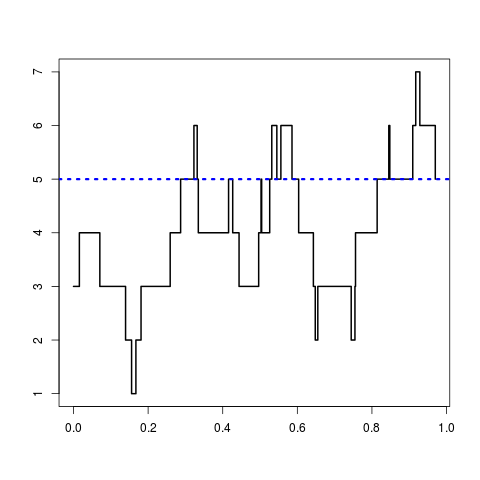
\includegraphics[height=.7\textheight, width=.7\textwidth]{../Figures/Fig-MinReg-BirDea-Thres} 
	 \onslide<2>    
	 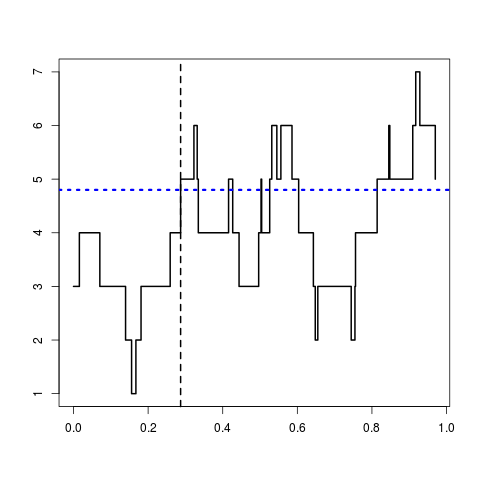
\includegraphics[height=.7\textheight, width=.7\textwidth]{../Figures/Fig-MinReg-BirDea-Time1}
	 \onslide<3>    
	 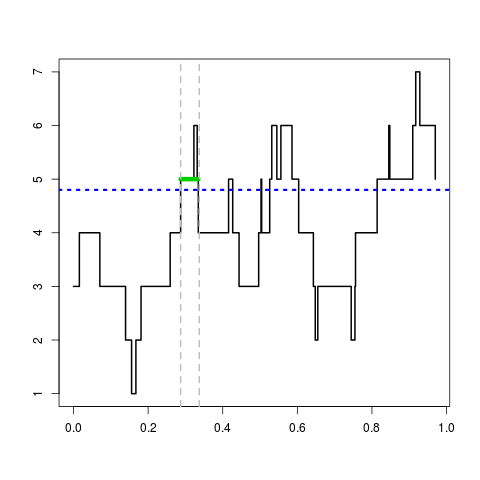
\includegraphics[height=.7\textheight, width=.7\textwidth]{../Figures/Fig-MinReg-BirDea-Excur1} 
	 \onslide<4>    
	 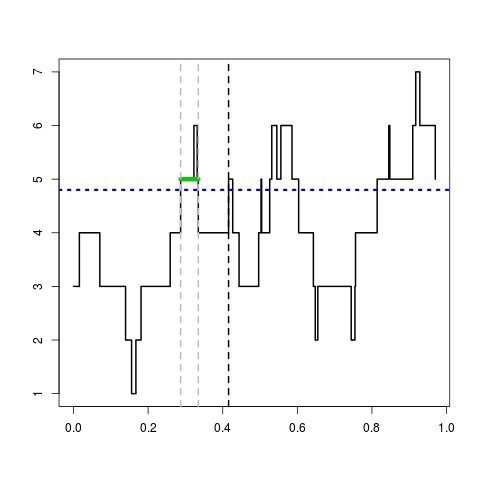
\includegraphics[height=.7\textheight, width=.7\textwidth]{../Figures/Fig-MinReg-BirDea-Time2} 
	 \onslide<5>    
	 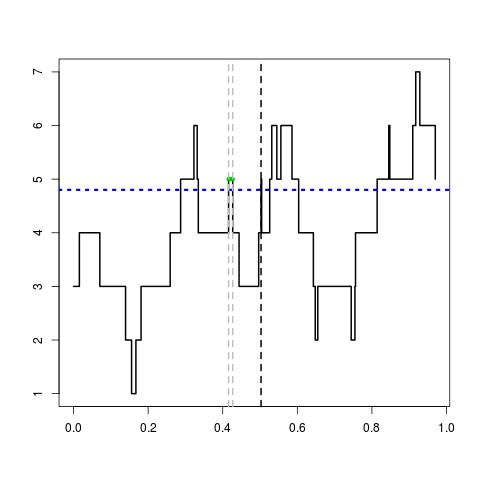
\includegraphics[height=.7\textheight, width=.7\textwidth]{../Figures/Fig-MinReg-BirDea-Time3} 
	 \onslide<6>    
	 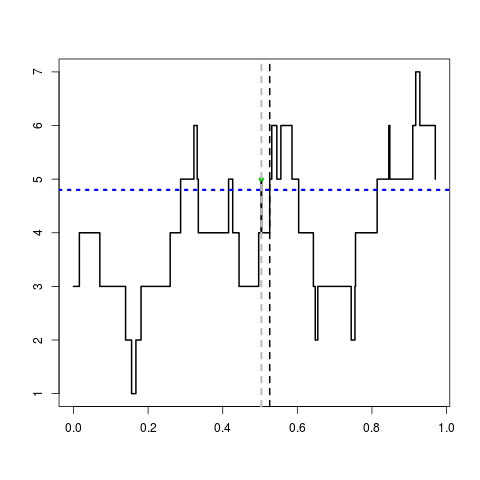
\includegraphics[height=.7\textheight, width=.7\textwidth]{../Figures/Fig-MinReg-BirDea-Time4} 
	 \onslide<7>    
	 \includegraphics[height=.7\textheight, width=.7\textwidth]{../Figures/Fig-MinReg-BirDea-Time5} 
	 \onslide<8->    
	 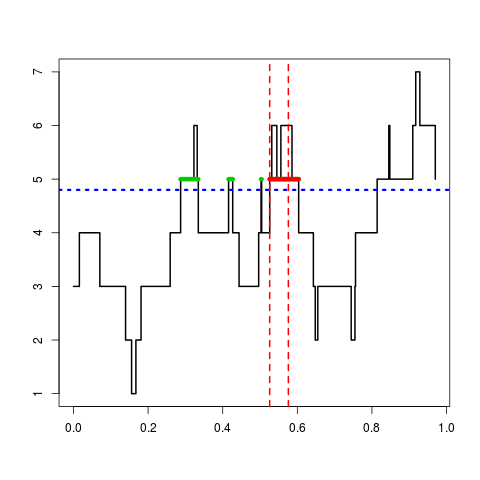
\includegraphics[height=.7\textheight, width=.7\textwidth]{../Figures/Fig-MinReg-BirDea-OK} 
	 \end{overprint} 
    \end{tabular}
  \end{tabular}
  \vspace{-.15\textheight}
  \begin{center}
  \onslide+<1->{$T(m, \ell) = $}
  \onslide+<2->{$A$} 
  \onslide+<3->{$+ B_1$} 
  \onslide+<4->{$+ C_1$} 
  \onslide+<5->{$+ (B_2 + C_2)$} 
  \onslide+<6->{$+ (B_3 + C_3)$} 
  \onslide+<7->{$+ (B_4 + C_4)$} 
  \onslide+<8->{$+ \ell$} \\   ~\\
  \end{center}
  \onslide+<8>{Number of trials $\sim$ geometric dist. with parameter $\Pr\{T_{m \rightarrow m-1} \geq \ell\}$}
  }

%====================================================================
\frame{\frametitle{Laplace transform}

  \paragraph{Reminder.} For a positive r.v. $X$, 
  $$
  \phi_X(u) = \Esp\left(e^{-uX}\right).
  $$
  \begin{itemize}
   \item for $X$ and $Y$ independent: $\phi_{X+Y}(u) = \phi_X(u) \phi_Y(u)$;
   \item for $(X_i)$ iid and independent from $Y$: $\phi_{\sum_{i=1}^Y X_i}(u) = \phi_Y\left(- \log \phi_X(u) \right)$;
   \item $\Phi_X(u) = \int F_X(x) e^{-ux} \dd x = \phi_X(u)/u$.
  \end{itemize}

  
  \bigskip \bigskip \pause
  \paragraph{Birth and death process.} 
  \begin{itemize}
   \item Hitting time: $T_{a \rightarrow b} = \inf\{t: S(t) = b | S(0) = a\}$.
   \item \refer{BaS01} provide the Laplace transform of hitting times $\phi_{T_{a \rightarrow b}}(u)$.
  \end{itemize}
}

%====================================================================
\frame{\frametitle{Laplace transform of the stopping time}

  \paragraph{Result.} Denoting $\phi_G$ the Laplace transform of $\mathcal{G}(1-q)$ [\footnote{$\phi_G(u) = (1-q) /(1 - q e^{-u})$}] where $q = \Pr\{ T_{m \rightarrow m-1} < \ell\}$, we have
  $$
  \phi_{T(m, \ell)}(u) = 
  \onslide+<2->{\phi_A(u)} 
  \onslide+<4->{\times \phi_G\left\{-\log [}
  \onslide+<3->{\phi_{B | < \ell}(u) \; \phi_C(u)}
  \onslide+<4->{] \right\}}
  \onslide+<5->{\times e^{-u \ell}}
  $$
  \onslide+<6->{and $\Phi_{T(m, \ell)}(u) = \phi_{T(m, \ell)}(u) / u$. }

  \bigskip \bigskip \bigskip \onslide+<7->{
  \paragraph{Practical calculation.} We are left with the inversion of $\Phi_{T(m, \ell)}$ to get 
  $$
  \Pr\{T(m, \ell) \leq n\} = \Phi^{-1}_{T(m, \ell)}(n),
  $$
  which can be done numerically using e.g. \refer{AbW06}.}
}

%====================================================================
\frame{\frametitle{(Provisional) conclusion}

  \paragraph{Ok:}
  \begin{itemize}
  \item Simple \& intuitive model,
  \item Exact result (up the continuous approximation).
  \end{itemize}

  \pause \bigskip \bigskip
  \paragraph{But:}
  \begin{itemize}
  \item The numerical inversion of $\Phi_{T(m, \ell)}$ is very instable \\
  \ra not usable in practice large population size $p$
  \end{itemize}

  }

%====================================================================
\section{Many loci, many patients}
\frame{\frametitle{Many loci, many patients}}
  
%====================================================================
\frame{\frametitle{Many loci, many patients}

  \paragraph{Mid 00':} NGS, DNA-seq
  \begin{itemize}
   \item $10^9$ nucleotides per genome, $10^7-10^8$ nucleotides per chromosome.
   \item Several tens of \EUR~per patient
  \end{itemize}
  
  \bigskip
  \paragraph{Data size:} 
  \begin{itemize}
   \item $n \rightarrow \infty$ loci
   \item $p \approx 10^3-10^4 \rightarrow \infty$ patients
  \end{itemize}
  
  \bigskip
  Joint work with L. Decreusefond\footnote{Ask me why TelecomParisTech is involved.}, M.-P. Etienne and G. Lang
}
  
%====================================================================
\frame{\frametitle{Convergence to a continuous process}

Same model as before, with an increasing number of patients $p$. 

\vspace{-.05\textheight}
\begin{center}
  \begin{tabular}{lc}
    \begin{tabular}{l}
    path of $\widetilde{S}_p(t)$: \\
    ~\\
    $p =$ 
    \onslide+<1->{10}\onslide+<2->{0}\onslide+<3->{0}\onslide+<4->{0} 
    \end{tabular}
    &
    \begin{tabular}{c}
	 \begin{overprint}   
	 \onslide<1>    
	 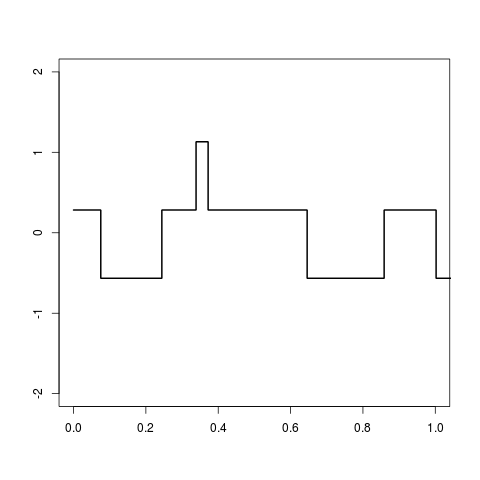
\includegraphics[height=.6\textheight, width=.6\textwidth]{../Figures/Fig-MinReg-Diffus-Cvg10} 
	 \onslide<2>    
	 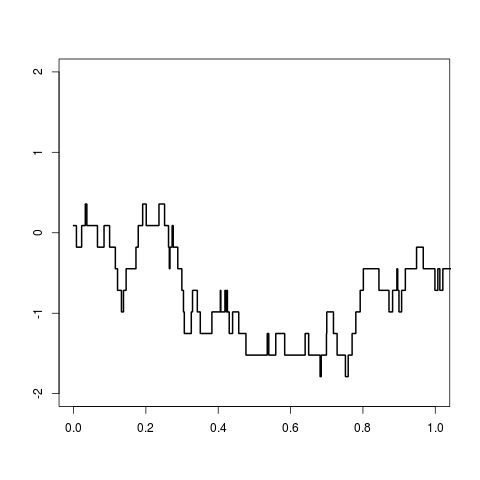
\includegraphics[height=.6\textheight, width=.6\textwidth]{../Figures/Fig-MinReg-Diffus-Cvg100} 
	 \onslide<3>    
	 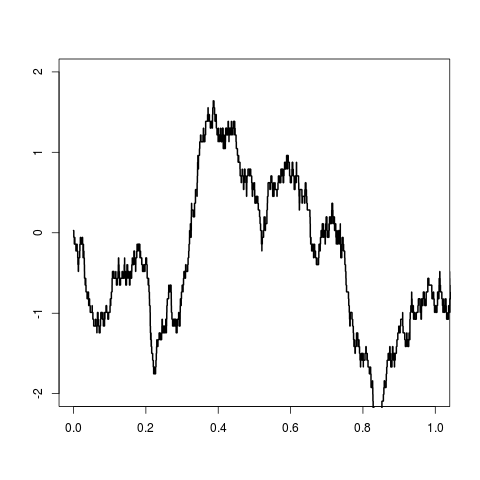
\includegraphics[height=.6\textheight, width=.6\textwidth]{../Figures/Fig-MinReg-Diffus-Cvg1000} 
	 \onslide<4->    
	 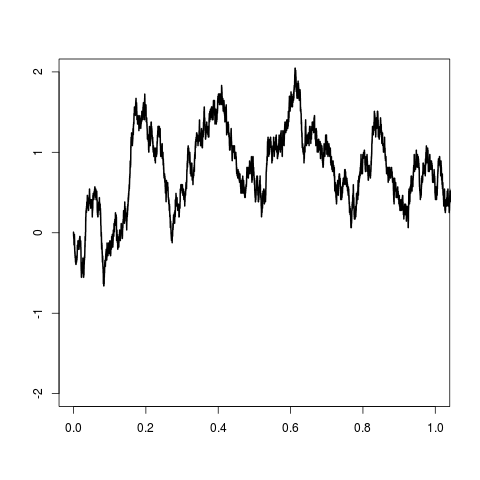
\includegraphics[height=.6\textheight, width=.6\textwidth]{../Figures/Fig-MinReg-Diffus-Cvg10000} 
	 \end{overprint}
    \end{tabular}
  \end{tabular} 
\end{center}
% \vspace{-.1\textheight}

\onslide+<4->
  {
  Paths of $S_p(t)$ becomes continuous as the number of patients $p \rightarrow \infty$.
  }
}

%====================================================================
\frame{\frametitle{Convergence to an Ornstein-Uhlenbeck (OU) process}

\vspace{-.05\textheight}
\begin{tabular}{cc}
  \begin{tabular}{p{0.4\textwidth}}
    \paragraph{Ornstein-Uhlenbeck process.} %Standard $OU(\tau) =$ Gaussian process $Z(t)$:
    \begin{itemize}
    \item Related to Brownian motion: $\dd \textcolor{red}{Z}(t) = e^{-\tau t} \dd B(t)$%: $Z(t) = e^{\tau t} \mathcal{N}(0, 1)/\sqrt{2} + \int_0^t \exp(-\tau t) \dd B(t)$ 
    \onslide+<2->{
    \item Possesses a stationary distribution (forced toward 0).
    }
    \end{itemize}
  \end{tabular}
  &
  \hspace{-.1\textwidth}
  \begin{tabular}{p{0.5\textwidth}}
    \begin{overprint}
     \onslide<1>
	 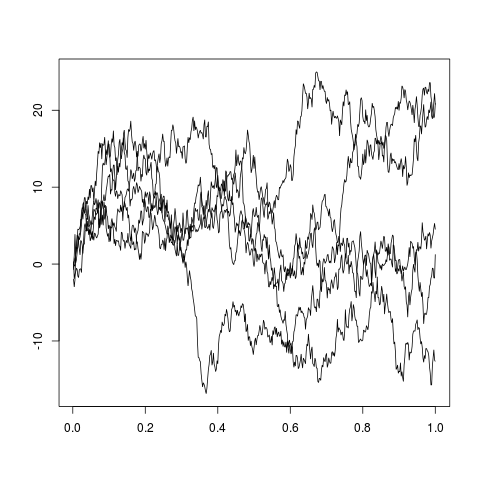
\includegraphics[height=.6\textheight, width=.6\textwidth]{../Figures/Fig-MinReg-Diffus-Bpaths} 
     \onslide<2->
	 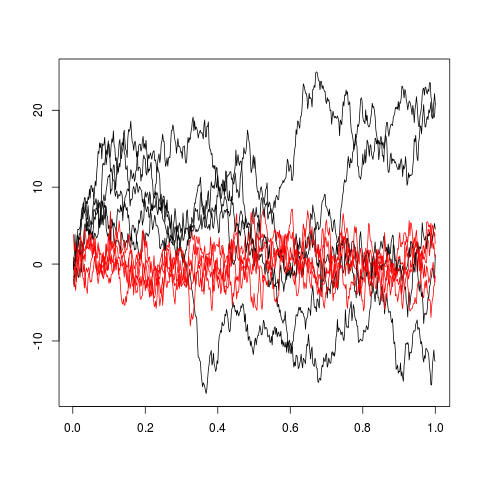
\includegraphics[height=.6\textheight, width=.6\textwidth]{../Figures/Fig-MinReg-Diffus-B-OUpaths}      
    \end{overprint}
  \end{tabular} 
\end{tabular}

% \paragraph{Ornstein-Uhlenbeck process.} %Standard $OU(\tau) =$ Gaussian process $Z(t)$:
% \begin{itemize}
%  \item related to the Brownian motion%: $Z(t) = e^{\tau t} \mathcal{N}(0, 1)/\sqrt{2} + \int_0^t \exp(-\tau t) \dd B(t)$
%  \item with a stationary distribution (recall toward 0).
% \end{itemize}

\vspace{-.05\textwidth} \onslide+<3->{
Denoting $\tau = \lambda + \mu$, $\theta = \lambda/\tau$, $\sigma^2 = \theta(1-\theta)$,
$$
\widetilde{S}_p(t) := \frac{S_p(t) - p \theta}{\sigma \sqrt{p}} 
\underset{p \rightarrow \infty}{\overset{\Delta}{\longrightarrow}}
OU(\tau)
$$
'$\Delta$' = convergence in distribution.}
}

%====================================================================
\frame{\frametitle{New problem}

  Denote $V_{OU}(\widetilde{m})$ the longest excursion\footnote{Of meanders and excursion: isn't it bucolic?} of an $OU(\tau)$ above threshold $\widetilde{m}$:
  $$
  \pi(m, \ell) = \Pr\{V_{OU}(\widetilde{m}) \geq \ell\}, \qquad \widetilde{m} = (m-p\theta)/\sigma\sqrt{p}.
  $$
  \vspace{-.075\textheight}
  \centerline{
%   \begin{tabular}{cc}
%     \begin{tabular}{p{0.4\textwidth}}
%     \end{tabular}
%     &
%     \hspace{-0.05\textwidth}
%     \begin{tabular}{p{0.5\textwidth}}
	 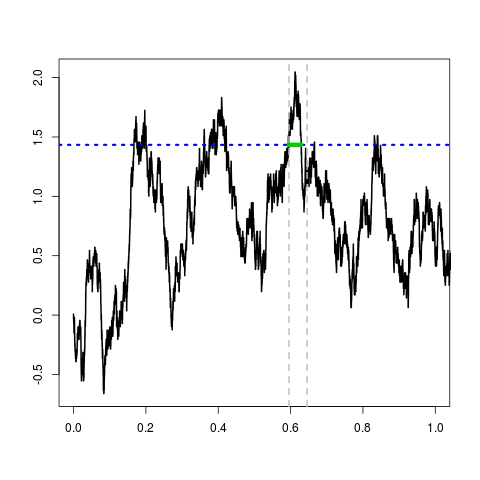
\includegraphics[height=.65\textheight, width=.7\textwidth]{../Figures/Fig-MinReg-Diffus-Longest} 
%     \end{tabular}
%   \end{tabular}
  }
  }

%====================================================================
\frame{\frametitle{Largest excursion}

  \paragraph{Orstein-Uhlenbeck process.} Very few is known.
  
  \bigskip\bigskip\pause
  \paragraph{Brownian motion.} \refer{PiY97} provide a (simple) way to sample the longest excursion $V^{(1)}_B$, the second longest $V^{(2)}_B$, ..., $V^{(n)}_B$, ... as a function of i.i.d. exponential variables $(U_1, U_2, ...)$:
%   can be sampled as follows:
%   \begin{enumerate}
%   \item Sample $(U_1, U_2, ...)$ i.i.d. $\sim \mathcal{E}(1)$,
%   \item Compute their cumulated sums: $C_n = U_1 + ... + U_n$,
%   \item Compute
  $$
  V^{(1)}_B = \frac{C_1^{-2}}{\sum_{j \geq 1} C_j^{-2}}, \quad
  V^{(2)}_B = \frac{C_2^{-2}}{\sum_{j \geq 1} C_j^{-2}}, \quad
  ...
  \text{ where } C_n = \sum_{j=1}^n U_j.
  $$
%   \end{enumerate}

  \bigskip\pause
  \paragraph{From Brownian excursions to OU excursions.}
  \begin{itemize}
   \item \cite{APP05} provide the distribution of the hitting time $T_{\widetilde{m}}$ for an OU process.
   \item The Girsanov formula for the rest of the path ($t > T_{\widetilde{m}}$) can be derived:
   $$
   \left.\frac{\dd P_{OU}}{\dd P_B}\right|_{\mathcal{F}_t} = f(V_B^{(1)}, V_B^{(2)}, ...)
   $$
  \end{itemize}
}

%====================================================================
\frame{\frametitle{Importance sampling}

\onslide+<1->
{We know how to sample $V^{(n)}_B$ but not \textcolor{red}{$V^{(n)}_{OU}$}. \\}

  \begin{tabular}{cc}
    \begin{tabular}{p{.4\textwidth}}
	 \begin{enumerate}
	 \onslide+<2->
	 {\item Sample a large number $N$ of copies $V^{(n)}_{B, 1}$, $V^{(n)}_{B, 2}$, ..., $V^{(n)}_{B, N}$. \\ ~}
	 \onslide+<3->
	 {\item Reweight each $V_{B, j}$ with 
	 $$
	 w_j \propto \textcolor{blue}{{\dd P_{OU}}/{\dd P_B}(V_{B, j})}.
	 $$}
	 \end{enumerate}
	 \onslide+<4->
	 {$$
	 \widehat{\pi}(m, \ell) = \frac{\sum_j w_j \mathbb{I}\{W_{B, j} > \ell\}}{\sum_j w_j}
	 $$}
    \end{tabular}
    &
    \hspace{-.05\textwidth}
    \begin{tabular}{c}
     \begin{overprint}
      \onslide<1>
     	 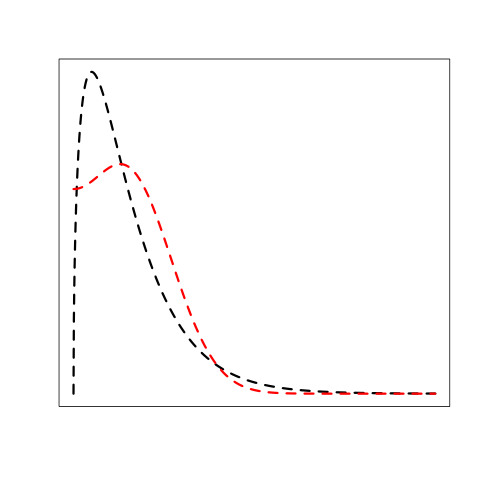
\includegraphics[scale=.4]{../Figures/Fig-MinReg-Diffus-ImpSamp0} 
      \onslide<2>
     	 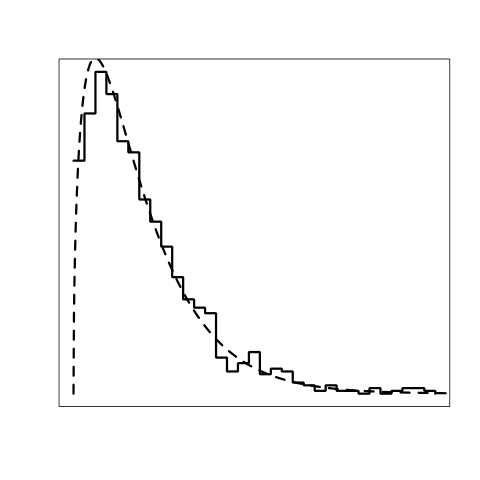
\includegraphics[scale=.4]{../Figures/Fig-MinReg-Diffus-ImpSamp2} 
      \onslide<3>
     	 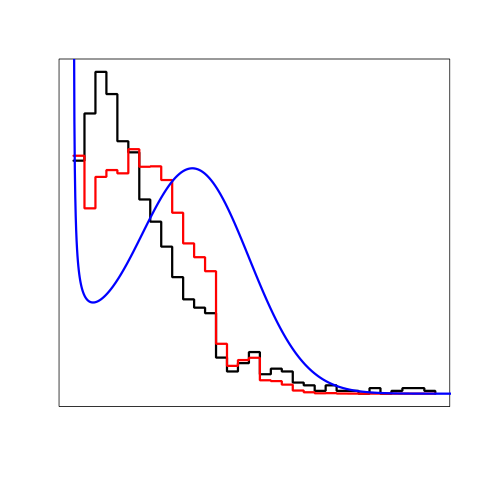
\includegraphics[scale=.4]{../Figures/Fig-MinReg-Diffus-ImpSamp3} 
      \onslide<4->
     	 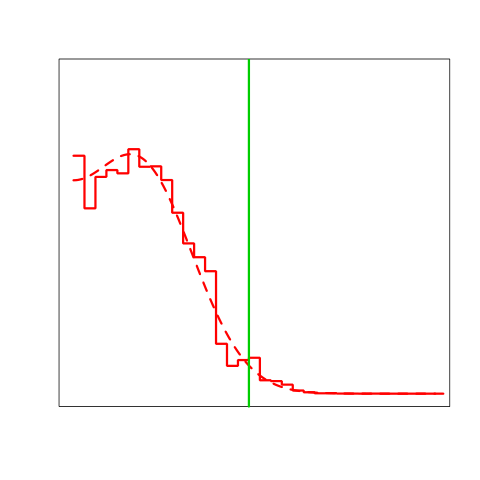
\includegraphics[scale=.4]{../Figures/Fig-MinReg-Diffus-ImpSamp4} 
     \end{overprint}
    \end{tabular}
  \end{tabular}
  
%   \vspace{-.05\textheight}
%   \onslide+<5>{A sampling scheme can be designed to sample $OU$ excursions.}

}

%====================================================================
\frame{\frametitle{A theoretical issue}

  \vspace{-.05\textheight}
  \begin{tabular}{cc}
    \begin{tabular}{p{.4\textwidth}}
	 \paragraph{The longest excursion} is not a continuous function so 
	 $$
	 \widetilde{S}_p \overset{\Delta}{\longrightarrow} OU(\tau)
	 $$
	 is not enough to prove that 
	 $$
	 V^{(1)}_{\widetilde{S}_p} \overset{\Delta}{\approx} V^{(1)}_{OU(\tau)}.
	 $$
    \end{tabular}
    &
    \hspace{-.1\textwidth}
    \begin{tabular}{c}
     	 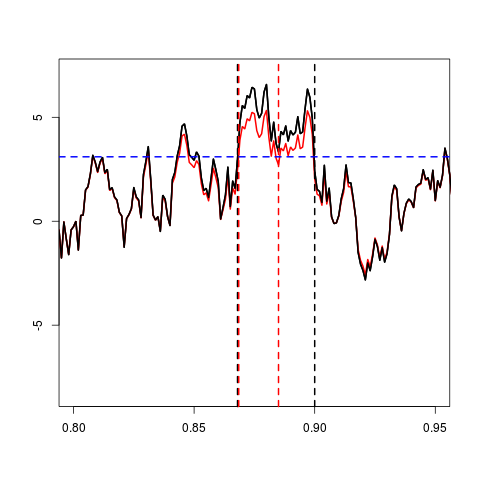
\includegraphics[width=.6\textwidth, height=.55\textheight]{../Figures/Fig-MinReg-Diffus-Continuity}      
    \end{tabular}
  \end{tabular} \\
  \pause
  Still, the problem can be reformulated as
  $$
  \pi(m, \ell) = \Pr\left\{\max_{\ell \leq t \leq T} \widetilde{S}_p^{-\ell}(t) \geq \widetilde{m}\right\}
  $$
  where $\widetilde{S}_p^{-\ell}(t) = \min_{t-\ell \leq u \leq t} \widetilde{S}_p(u)$, which relies on continuous transforms\footnote{Many thanks to P. Vallois.}.
  
%   $\widetilde{S}_p \overset{\Delta}{\longrightarrow} OU(\tau)$
%   means that, for any continuous function $f$:
%   $$
%   \mathbb{E}[f(\widetilde{S}_p)] \underset{p \rightarrow \infty}{\longrightarrow}  \mathbb{E}[f(OU(\tau))].
%   $$
%   \vspace{-.05\textwidth}
%   \begin{tabular}{cc}
%     \begin{tabular}{p{.4\textwidth}}
% 	 \paragraph{The longest excursion} of $\widetilde{S}_p$ above $\widetilde{m}$ is a (measurable) function ... \\
% 	 ~\\
% 	 but it is not continuous.
%     \end{tabular}
%     &
%     \hspace{-.05\textwidth}
%     \begin{tabular}{c}
%      	 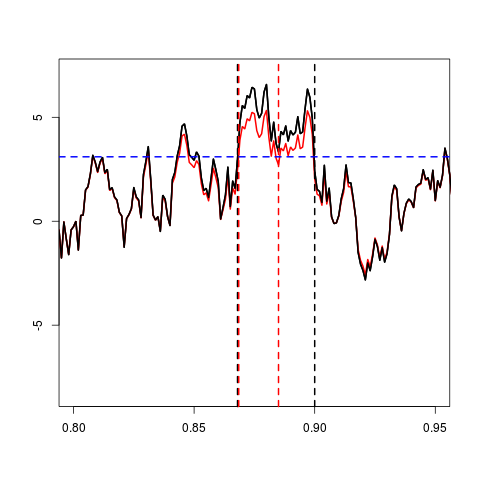
\includegraphics[scale=.4]{../Figures/Fig-MinReg-Diffus-Continuity}      
%     \end{tabular}
%   \end{tabular}

}

%====================================================================
\frame{\frametitle{(Provisional) conclusion}

  \paragraph{Ok:}
  \begin{itemize}
  \item The approximation can handle arbitrarily loci density and number of patients \\
  \ra 'scalable' approach for next sequencing technologies ($n \approx 10^8$)
  \item Abacus can be computed once for all.
  \end{itemize}

  \pause \bigskip \bigskip
  \paragraph{But:}
  \begin{itemize}
  \item The proposed sampling strategy still needs to be implemented in practice...
  \item The efficiency of the preferential sampling scheme is critical.
%   \item   We have no theoretical guarantee that the longest excursion of the process of interest behaves like this of an Ornstein-Uhlenbeck process.
%   \item In the worst case, the proposed approach is useless.
  \end{itemize}

  }

%====================================================================
\frame{\frametitle{General conclusion}

  \paragraph{Running after technologies.}
  \begin{itemize}
  \pause
  \item Each new technology provides new (statistical) problems. \\ ~
  \pause
  \item Many of them are related to artifact correction \\
  \ra Statistical developments become rapidly obsolete.  \\ ~
  \pause
  \item Some are more rewarding: \\
  \ra they raise interesting theoretical problems \\
  \ra to provide answers to practical questions. 
  \end{itemize}

}

%====================================================================
{\tiny
  \bibliography{/home/robin/Biblio/ARC,/home/robin/Biblio/AST,/home/robin/Biblio/SSB}
  \bibliographystyle{/home/robin/LATEX/Biblio/astats}
%   \bibliographystyle{ieeetr}
  }


%====================================================================
%====================================================================
\end{document}
%====================================================================
%====================================================================
